
\lhead[\chaptername~\thechapter]{\rightmark}

\rhead[\leftmark]{}

\lfoot[\thepage]{}

\cfoot{}

\rfoot[]{\thepage}

\chapter{Faster ANN}
\label{FasterANN}

\section{Method}

\begin{figure}
    \centering
    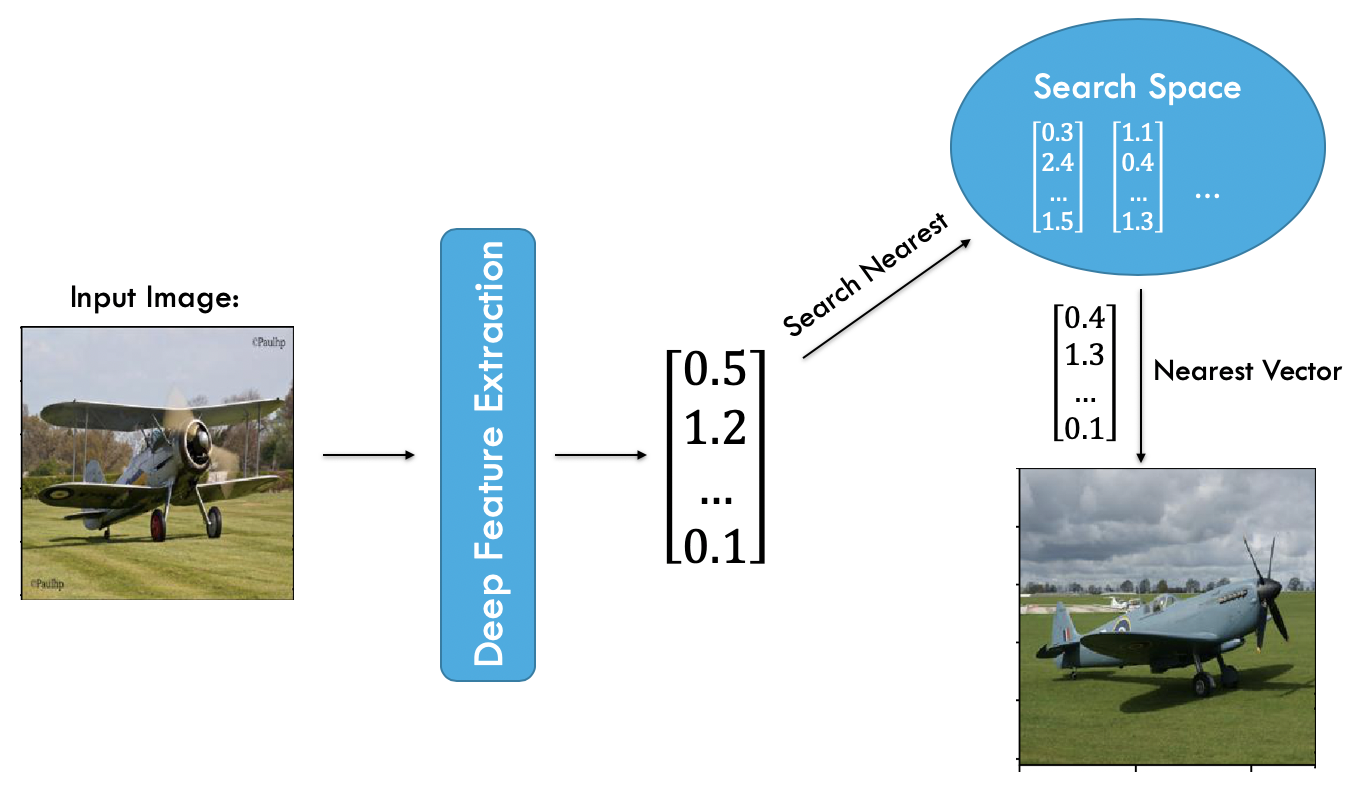
\includegraphics[width=0.9\textwidth]{thesis/images/image_ret_exp-fig.png}
    \caption{Overview of Image Retrieval}
    \label{fig:ret-exp}
\end{figure}

In image retrieval task, images are represented as vectors and the aim is to search a database of vectors for the nearest vector to the input image, as in figure \ref{fig:ret-exp}. 
For each query vector $\mathcal{Q} = \{\bm{q}_1,\bm{q}_2,\dots\} \subset \mathbb{R}^D$ and database vectors $\mathcal{X} = \{\bm{x}_1, \dots, \bm{x}_N\} \subset \mathbb{R}^D$, the task is to retrieve the most similar image with $n^* = \underset{n\in\{{1,\dots,N}\}}{\mathrm{argmin}} \vert\vert \bm{q} - \bm{x_n} \vert\vert $ for each query vector. 

Naive approach would be brute-force searching the entire database.
However, exhaustive searching of the database is slow and costly, especially with vectors with large dimensions. 
Thus, Approximate Nearest Neighbor (ANN) search algorithms are proposed with significantly faster search speed and a small probability of error. 
We built our work on the FAISS implementation~\cite{faiss} of Product Quantization~\cite{jegou2010product} with inverted multi-index as well as using it as our baseline.

As explained in section \ref{subsec:related-quantization}, product quantization method clusters the database space into $K$ clusters using k-means algorithm, $\mathcal{X}_1,\dots,\mathcal{X}_K$ where $\bigcup_{i=1}^K \mathcal{X}_i = \mathcal{X}$ and $\mathcal{X}_i \bigcap \mathcal{X}_j = \emptyset$. 
We will refer to these clusters as subspaces or cells.
Then, the database vectors are assigned into one of $\mathcal{X}_k$.
When a query vector $\bm{q}\in\mathbb{R}^D$ is searched, first the nearest $\mathcal{X}_k$ is retrieved. 
Then, all vectors $\bm{x}\in\mathcal{X}_k$ is traversed to find the nearest vector.

Our work aims to reduce the area of the search space by limiting the number of comparisons in the first step with $\mathcal{X}_k$ for each user according to their requirements. 
ANN search algorithms commonly assume that the distribution of the query vectors is the same with the distribution of the database vectors. 
However, real users have diverse query distributions, different than that of the database, 
so they query some parts of the search space more and the other parts less likely. 
This difference is sourcing from their limited surroundings in daily life or their different hobbies and interests. 
By utilizing this idea, we can reduce the search space by limiting the comparisons only to the relevant $\mathcal{X}_k$ for each user according to their requirements.

\begin{figure}
    \centering
    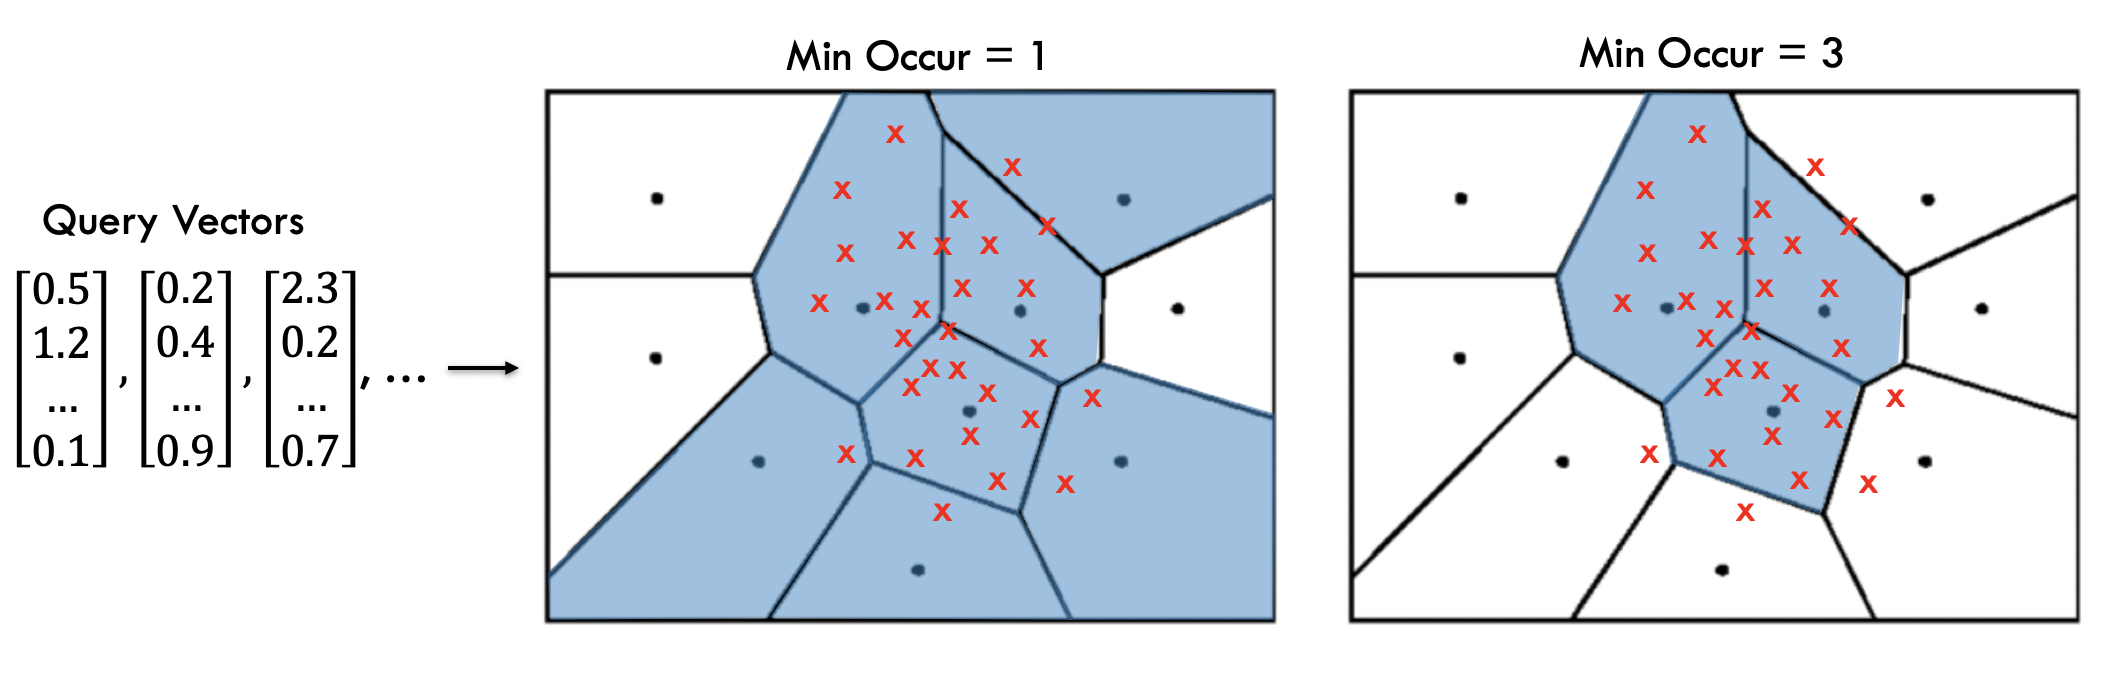
\includegraphics[width=\textwidth]{thesis/images/improvement-fig.png}
    \caption{Query vectors and clustering of the search space is shown. Red crosses represent the position the query vectors fall in the space. We can choose to include every subspace with red crosses in our search as in the left figure. A hyper-parameter can control to include a subspace according to minimum occurrence of red crosses.}
    \label{fig:motivation}
\end{figure}

In figure \ref{fig:motivation}, query image examples of a user is shown with red crosses on the search space. 
For this user, a new query vector just needs to be compared with centroids in blue areas. 
We can reduce the amount of centroids to compare with a simple hyper-parameter, controlling whether to include a subspace according to minimum occurrence of the past query vectors. 
In this way, we can adjust the trade-off between accuracy and the speed of the system.

In the following subsections, our work will be explained in detail. 
Firstly, the details of using classification label information to reduce the area of search space will be explained. 
Next, the dataset and the distribution of class labels to subspaces will be discussed.
Then, the method of representing the images with vectors will be described in detail. 
After specifying the implementation details, baselines of our work will be defined.

\subsection{Using classification label information}

In our method, we used classification labels to represent the user requirements. 
Given the classification labels $\mathcal{C} = \{1,2,\dots,C\}$ where $C$ is the number different of labels, each user requirement is defined as $\mathcal{U} \subseteq \mathcal{C}$. 
Assuming we know the classification labels of our database vectors, $\mathcal{X}$ can be redefined as $\mathcal{X} = \{(\bm{x_1}, c_1), \dots, (\bm{x_N}, c_N)\}$.
Then, the subspaces will also contain the class labels, $(\bm{x}, c) \in \mathcal{X}_k$.

Given a user requirement $\mathcal{U}$ to our system, we choose the corresponding subset of all subspaces according to the following algorithm.
If any of $(\bm{x}, c) \in \mathcal{X}_k$ contains the class label $c \in \mathcal{U}$, we consider that subspace as a relevant subspace to our user.
Let us define the relevant subspaces as $\mathcal{X}_\mathrm{rel} \subseteq \{\mathcal{X}_1,\dots,\mathcal{X}_K\}$.

In the search part of our algorithm, the query vector $\bm{q} \in \mathbb{R}^D$ is compared with the representative vectors of $\mathcal{X}_\mathrm{rel}$ instead of all the $\{\mathcal{X}_1,\dots,\mathcal{X}_K\}$. 
The remaining part of our algorithm is the same with the original PQ method.
Once the nearest $\mathcal{X}_k$ is found, the vectors associated with that subspace are traversed to find the nearest vector.

Our method accelerates the coarse quantization part of the PQ algorithm, where finding the closest subspace is the objective. 
We show the significance of accelerating the first part of PQ as the following.
Following the convention, we chose $K=\sqrt{N}$ where $N$ is the number of database vectors. 
In this way, number of vectors corresponding to $\mathcal{X}_k$ will be $\sqrt{N}$ in average. 
Once a query vector comes, the algorithm searches the closest centroid among $\sqrt{N}$ centroids. 
Then, the query vector is compared with the database vectors that belong to the chosen $\mathcal{X}_k$ and a few neighboring ones. 
In both steps, there are $O(\sqrt{N})$ comparisons to be done. 
Therefore, accelerating the first part is as important as accelerating the second part.

\subsection{Dataset and Distribution of Class Labels to Subspaces}
\label{retrievallabelinfo}

In our experiments, we used the scene recognition dataset called Places365~\cite{zhou2017places}. 
There are 1.8 million training images with 365 class categories. 
1.3 million out of all images is used to construct our search database. The remaining images are used to train the ANN algorithm and also for the query vectors.
The class categories include various scenes such as airport terminal, library, train station, waterfall, etc. 
With such diverse scenes, users would interact with only a subset of the class categories and our idea can be easily applied to speed up the search according to each user's requirements.

\begin{figure}
    \centering
    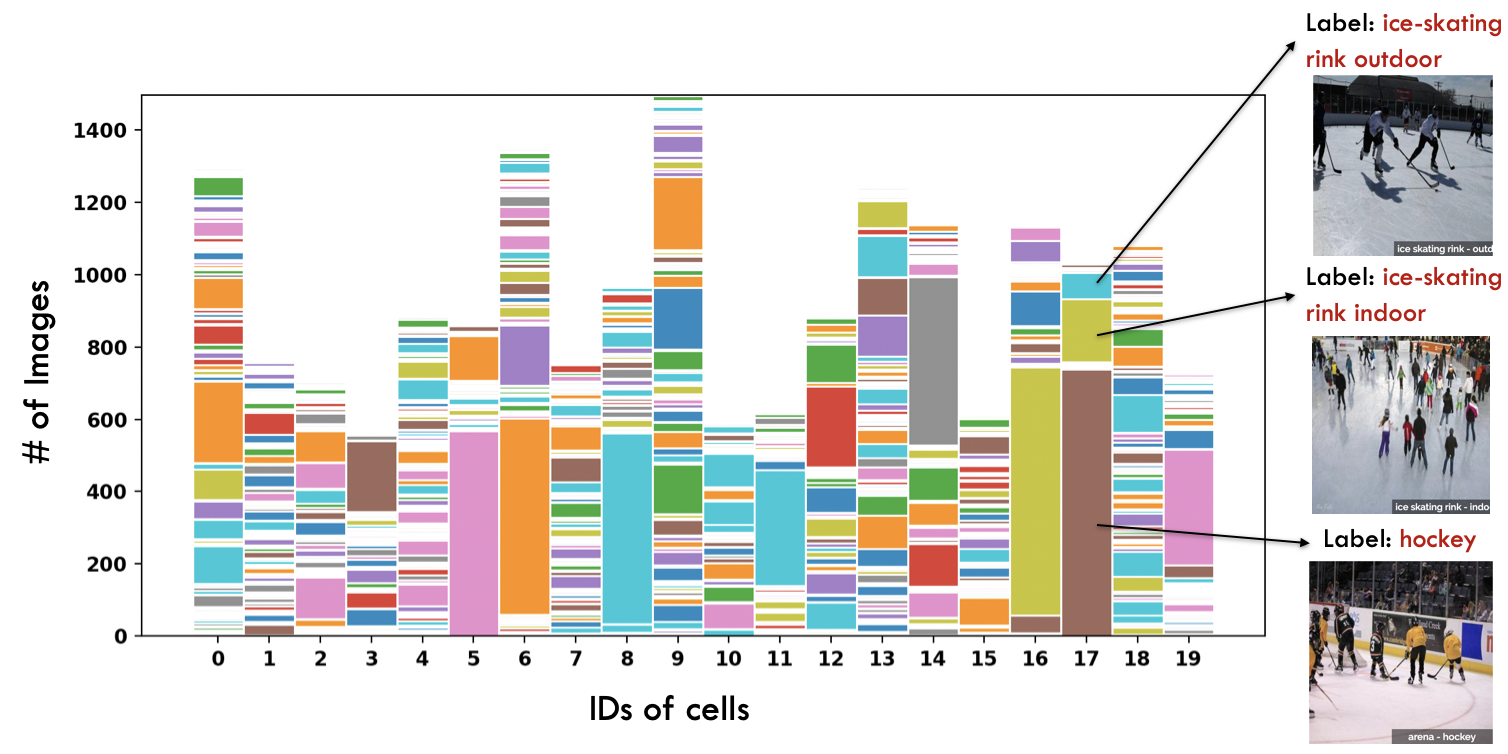
\includegraphics[width=\textwidth]{thesis/images/label_dist-fig.png}
    \caption{Distribution of the images according to their class labels in the first 20 subspaces}
    \label{fig:label-dist}
\end{figure}

Following the convention, we chose the number of subspaces as $K=\sqrt{N}$ where $N$ is the number of database vectors. 
Therefore, the search space is divided into 1140 subspaces which is the square root of the number of images($\sqrt{N}$) in our search database. 
Distribution of the images to those subspaces according to their classification labels can be seen in the figure \ref{fig:label-dist}.
As can be seen in the figure, some subspaces have extreme bias towards a few class, while others do not have much. 
There are many class categories in Places dataset that have similar images, such as "elevator-door", "elevator-interior", "elevator lobby", "elevator shaft", etc.
For example, the subspace with id:17 in the figure has labels with very similar images.


\subsection{Extracting Deep Features of Images}
\label{extractdeepfeatures}

\begin{figure}
    \centering
    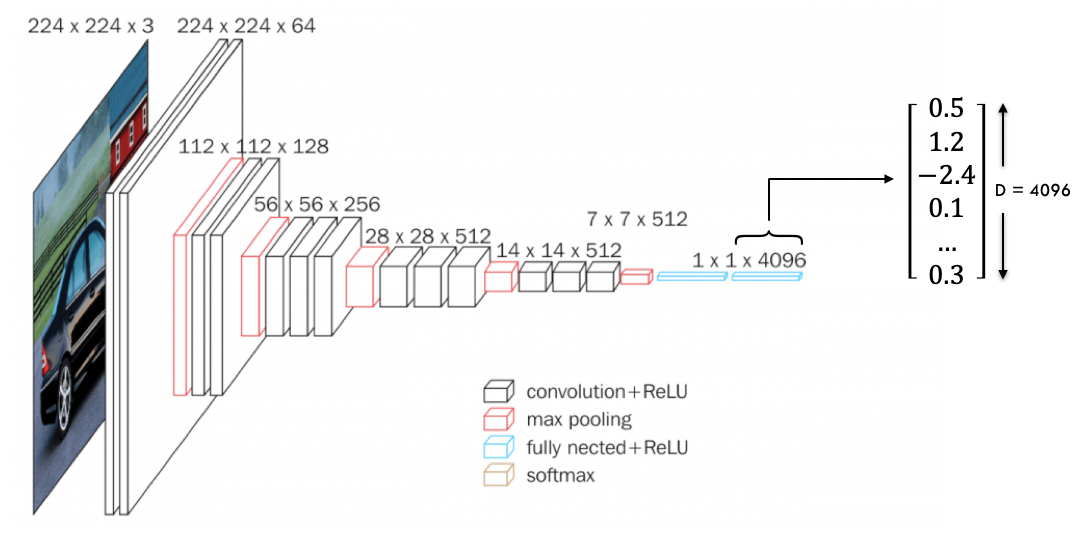
\includegraphics[width=0.9\textwidth]{thesis/images/deep_features-fig.png}
    \caption{Last fully connected layer of VGG16~\cite{simonyan2014very} is discarded to obtain a descriptor vector with dimension 4096.}
    \label{fig:vec-repr}
\end{figure}

In the work of Babenko \emph{et al.}~\cite{babenko2014neural}, using a pre-trained convolutional neural network in ImageNet for image retrieval task is shown to have decent results. 
Note that, it is also shown that if the network is trained on the same data with the retrieval dataset, the results are better.
However, instead of getting the best performance, we simply investigate the comparison of our idea with the current best methods.
Therefore, we used VGG16~\cite{simonyan2014very} network that is pre-trained on ImageNet~\cite{deng2009imagenet}. 
The last fully connected layer is discarded to get a vector representation with 4096 dimensions, as in figure \ref{fig:vec-repr}.
Then, all database images are passed through the model once to get their descriptor vectors.

However, dimensions of the vectors were quite big for both storage and calculation. 
As stated in \cite{jegou2012negative}, applying whitening on the descriptor vectors not only helps with the computational and storage costs, but also improves the accuracy of retrieval tasks.
We applied Principal Component Analysis (PCA) to obtain the final descriptor vectors with 64 dimensions.


\section{Experiments}

\subsection{Implementation Details}

As mentioned before, we built our work on FAISS implementation~\cite{faiss} of product quantization with inverted index, namely IndexIVFPQ. 
The code is shared publicly and we modified the code to tailor to our needs.
Extra function is added to adjust the search space according to a given list. 
This function is called during the indexing phase of the database before the search.

The training phase is required for IndexIVFPQ and it needs different vectors than the database vectors with similar distribution.
Training dataset of Places365 contains 1.8 million images. 
After obtaining the descriptor vectors of the images, we split the vectors into three parts.
Base vectors containing roughly 1.3 million vectors to form the search space, about a half million training vectors to train IndexIVFPQ and remaining approximately 3000 for query vectors.
The vectors are split into 3 parts in a way that the number of images for each label in all parts are almost equal.
When querying for a user, only the images with the required labels out of 3000 are used for the query images.

\subsection{Baselines}

Our main baseline is the FAISS implementation~\cite{faiss} of product quantization with inverted index, namely IndexIVFPQ.
We compared our method with IndexIVFPQ by evaluating both method for search time per query and recall at 1 where recall at $k$ checks if the true result is one of the $k$ predicted results. 

\subsection{Experiments}

\begin{figure}
    \centering
    \begin{minipage}[b]{.5\textwidth}
        \centering
        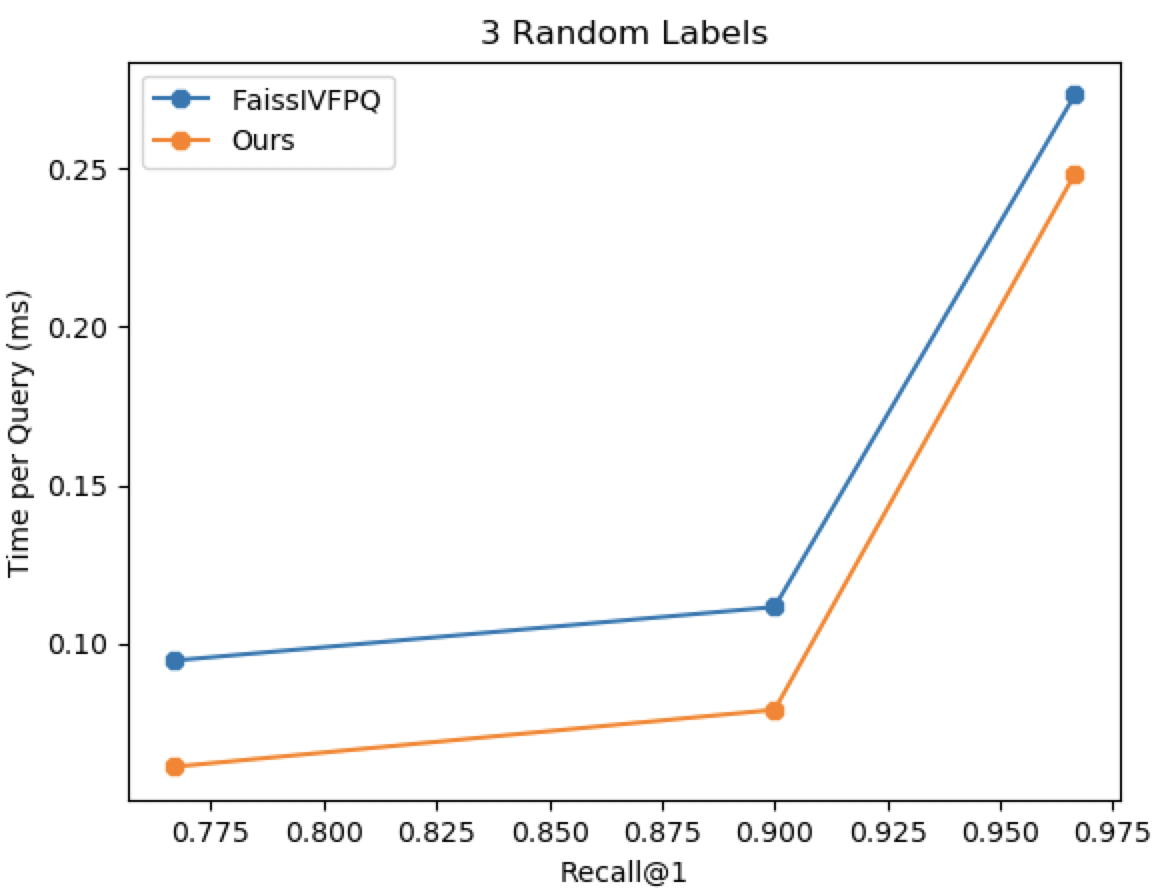
\includegraphics[width=.9\linewidth]{thesis/images/3_random.png}
        % \caption{Results for 3 random label}
        \label{fig:randomexpsub1}
    \end{minipage}%
    \begin{minipage}[b]{.5\textwidth}
        \centering
        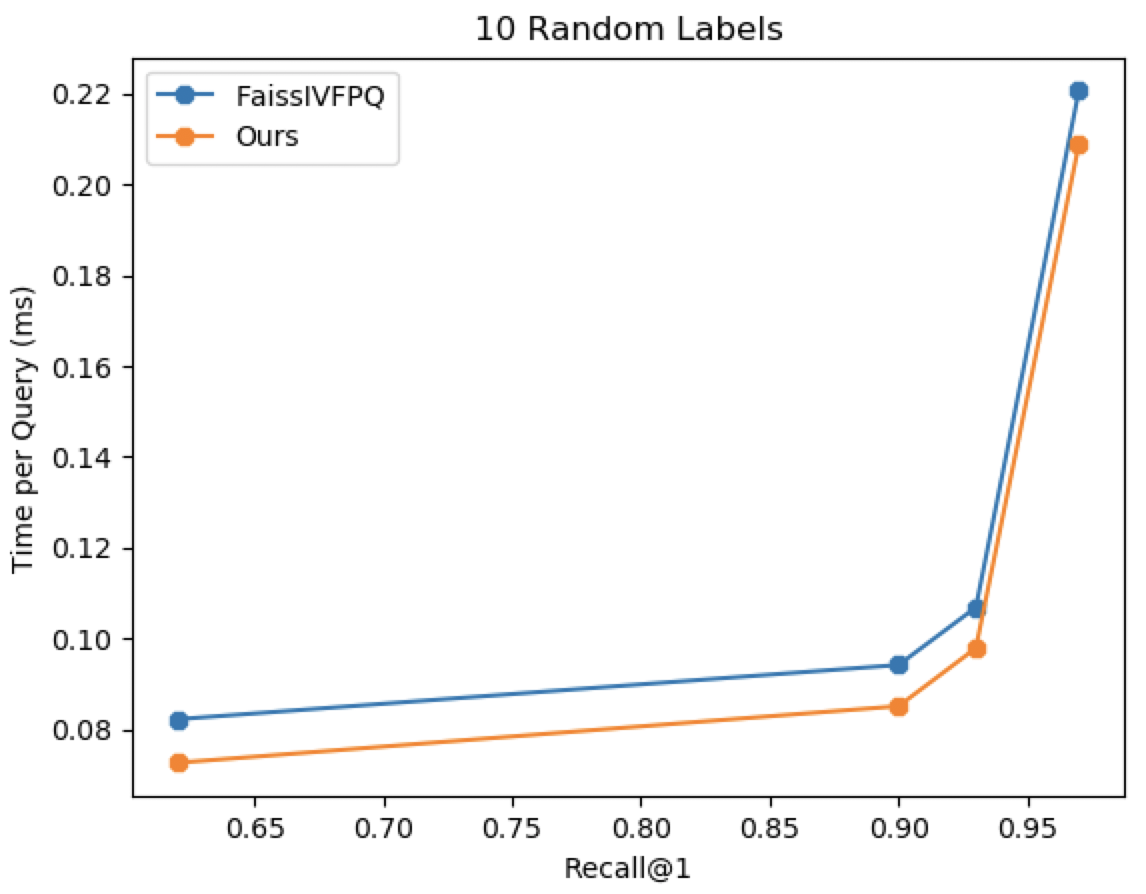
\includegraphics[width=.9\linewidth]{thesis/images/10_random_only_mo1.png}
        % \caption{Results for 10 random label}
        \label{fig:randomexpsub2}
    \end{minipage}
    %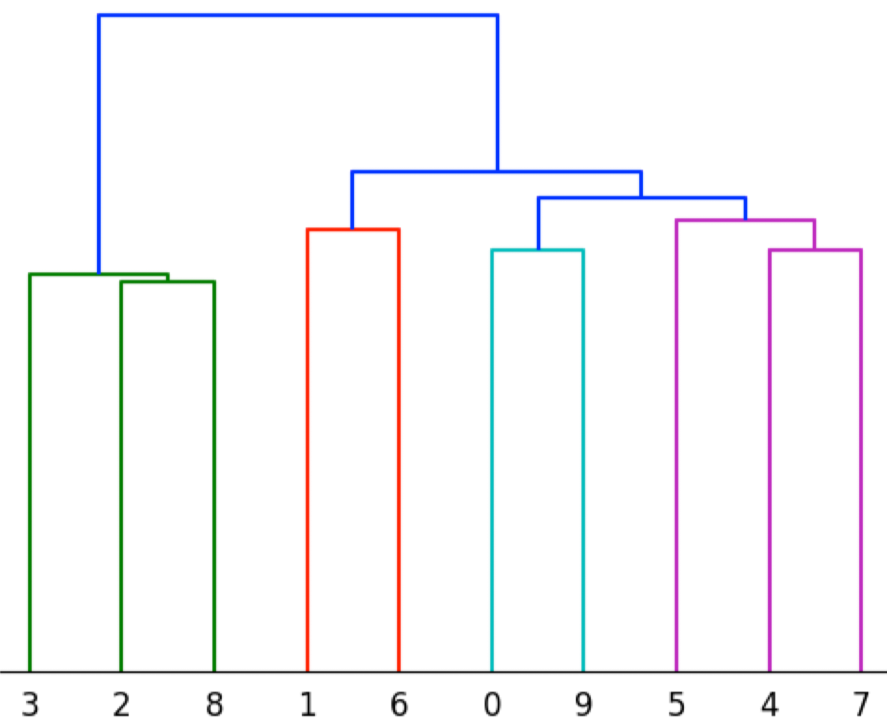
\includegraphics[width=0.40\textwidth]{images/hierfig.png}
    \caption{Comparison of our method with FaissIVFPQ on randomly picked labels as user requirements}
    \label{fig:randomexp}
\end{figure}

According to our scenario, users have wearable devices with a camera, such as wearable glasses or a smart phone. 
When they first start using the image search system, the class recognition system will store the classification labels of the users. 
After storing labels for enough time, we will consider those labels as the user's required class labels.
Then, we select the subspaces, out of all 1140 subspaces, that contain any of those class labels at least $m$ times. 
$m$ is the hyper-parameter to adjust the trade-off between accuracy and speed.
Whenever a new query image comes from the user, we compare the query vector only with the centroids of the selected subspaces to reduce time.
Note that, classification labels are merely a tool for us to categorize the requirements of the users.
Most similar images do not necessarily have the same labels.

In our experiments, two types of tests are conducted. 
The first phase of testing is done with random or hand-picked data to analyze our method thoroughly. 
For the second phase of testing, real data is used to observe whether our method is applicable to real-life scenarios. 
Two phases will be explained in their respective sections.

\subsubsection*{Experiments with Artificial Data}

\begin{figure}
    \centering
    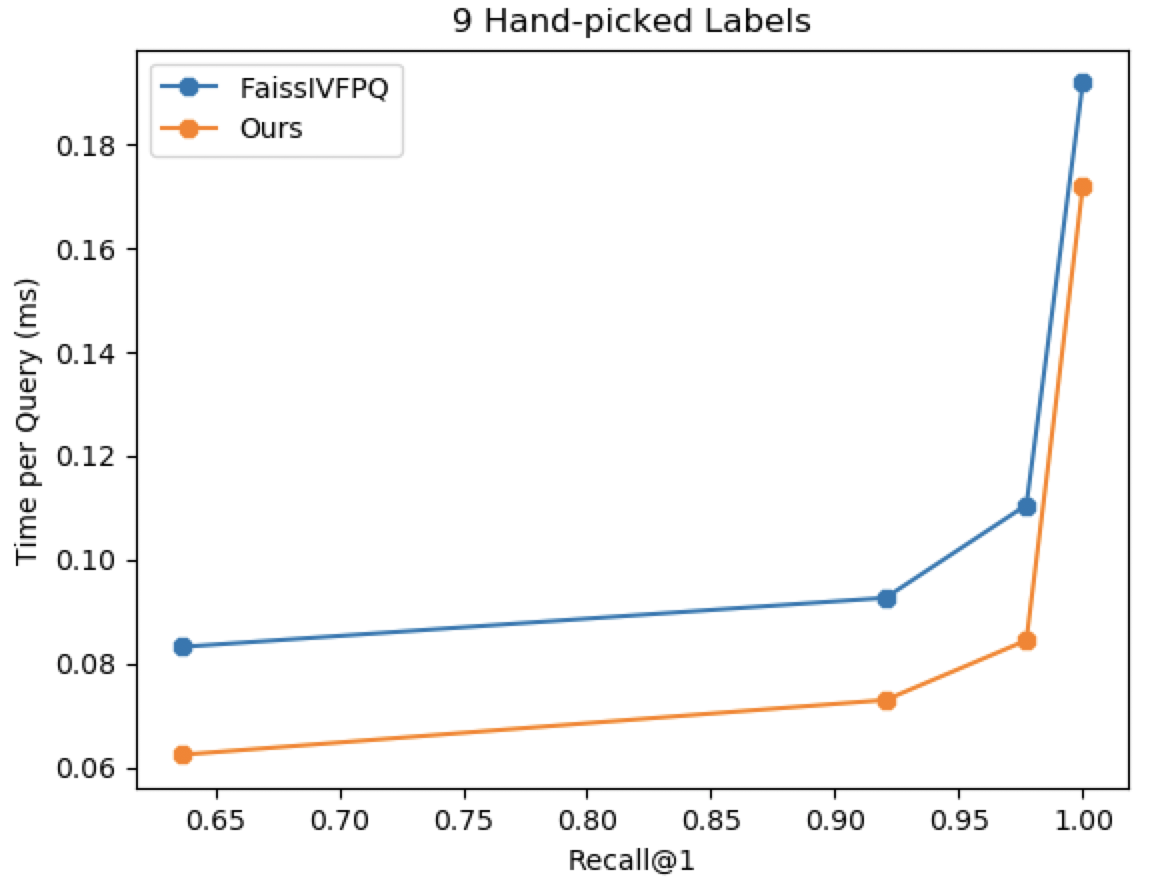
\includegraphics[width=0.8\textwidth]{thesis/images/9_handpicked.png}
    \caption{Comparison of our method with FaissIVFPQ on hand-picked labels as user requirements}
    \label{fig:handpickedexp}
\end{figure}

Our proposed method is making use of the user requirements to speed up the search for image retrieval. 
In our work, user requirements are represented with the classification labels. 
These are the labels that the users most likely encounter in their daily lives. 
According to our scenario, these labels are extracted with a recognition model included in their device as mentioned earlier in \ref{retrievallabelinfo}. 
In our experiments, we either randomly picked or hand-picked these labels to validate our method with diversified tests.

When the class labels are randomly picked, the results are expected to be the worst for our method. 
The reason is that randomly picked labels would not be related to each other, whereas in real life user-required labels might have similar images. 
Because the task is similarity search, similar images with different labels are closer in the search space, therefore it is easier to reduce the space more.
For example, randomly picked labels might include labels such as volcano, waterfall, ski slope at the same time, whereas user-required labels are more likely to have labels such as campus, library-outdoor, library-indoor.
Having said that, results for randomly picked labels can be seen in the figure \ref{fig:randomexp}.
In both of the figures, it can be clearly seen that our method surpasses the baseline as our method can perform faster with the same accuracy.

Further experiments are done with hand-picked labels. 
In these experiments, labels are picked intuitively considering their relevancy. 
The results can be seen in the figure \ref{fig:handpickedexp}. 
We can see again that our method performs better than the baseline.
Note that points in the graphs are taken by changing the nprobe parameter. 
After finding the closest subspace to the query vector, the algorithm searches for a few neighboring ones. 
The number of subspaces to check is controlled with nprobe.


When the number of labels chosen for user requirements is relatively small, our method outperforms the baseline method.
However, as the number of labels go up, our method starts to behave similarly to the baseline.
The reason is that we only search the sub-spaces in our search space which contains at least $k$ of any required labels. 
When the number of labels is high, it becomes harder to exclude some sub-spaces. Because almost all of them has at least one of any required labels. 
That is why, our method works if user required labels are relatively small which actually makes sense because if the user requires many labels, they do not need to use our system as they can use generic model for their need.


\subsubsection*{Experiments with Real Data}

\begin{figure}
    \centering
    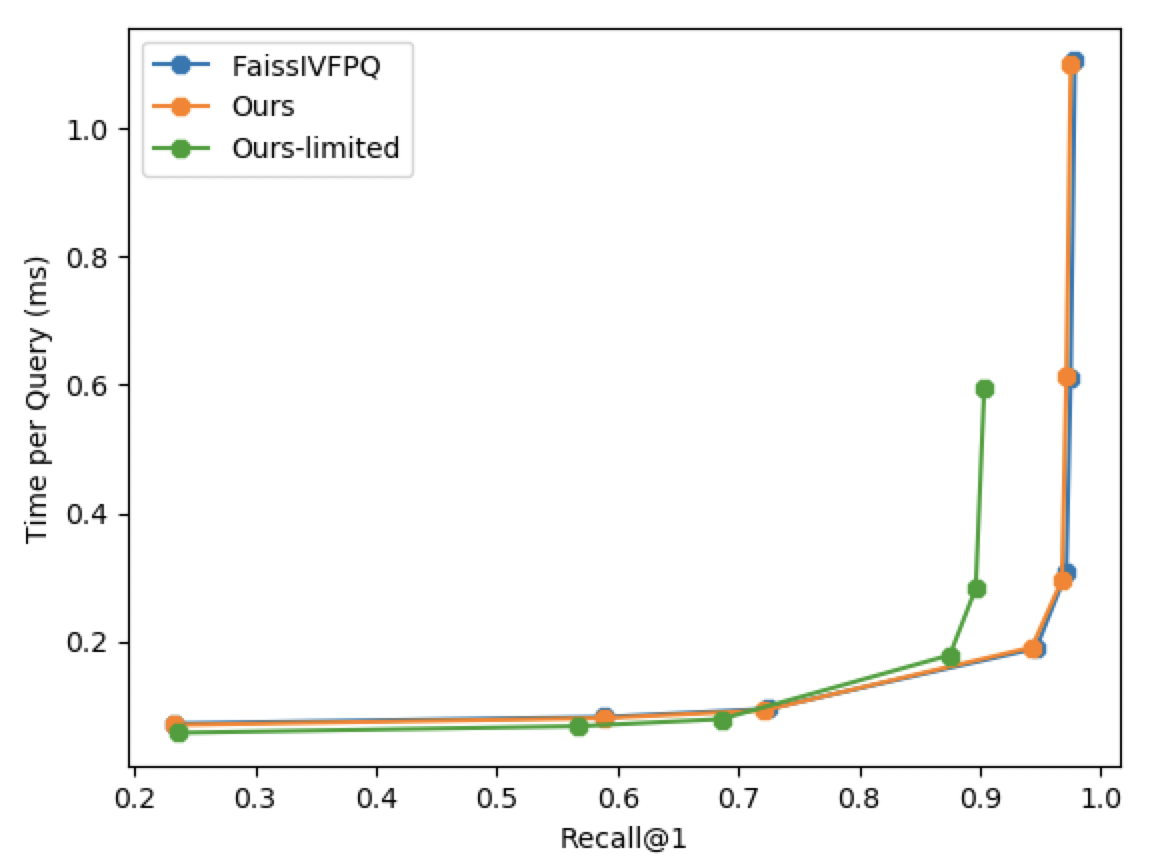
\includegraphics[width=0.8\textwidth]{thesis/images/real_data_experiment.png}
    \caption{Comparison of our method with FaissIVFPQ in a real-life experiment}
    \label{fig:realdataexp}
\end{figure}

The real data for this phase is obtained using GoPro Hero8 with a chest mount. 
Daily v-logs are taken for 2 days, first day data is used for extracting user required classification labels and second day data is used to actually test our method.

Daily v-logs are recorded for 2 days for nearly a total of 2 hours. 
Videos are mostly taken when the subject is on the move to prevent recording constant same scenes.
For each day, videos are sampled with a ratio of 1 frame per 10 seconds. 
426 frames for the first day and 280 frames for the second day is obtained.

First day frames are classified with a pre-trained ResNet with 18 layers~\cite{resnet}. 
73 different labels are recognized from 426 frames with many misclassified labels such as airplane cabin, airport terminal, berth, catacomb and many more. 
Many labels are predicted only once or with little probabilities. Therefore, a limit is put to probability and minimum occurrence to exclude some of the labels. 
We refer to this method as "Ours-limited".

Second day frames(280) are converted to query vectors with the usual process, explained in \ref{extractdeepfeatures}. The result of searching with these query images is shown in the figure \ref{fig:realdataexp}. 
There are 1140 sub-spaces in the search space. Our method could reduces the area to only 1108 sub-spaces using 73 user-required labels. 
Thus, our method fails to speed up the baseline for the real-life experiment. 
Limited version of our method is obtained by a limit to probability by 50 percent classification accuracy and at least 3 minimum occurrence of labels to count them as requirements.
However, excluding some classified labels reduced the accuracy of "Ours-limited".
Results will be discussed more thoroughly in the next chapter and further experiment results will be shown in \ref{Appen} Additional Results.

